% Options for packages loaded elsewhere
\PassOptionsToPackage{unicode}{hyperref}
\PassOptionsToPackage{hyphens}{url}
\PassOptionsToPackage{dvipsnames,svgnames*,x11names*}{xcolor}
%
\documentclass[
  11pt,
]{article}
\usepackage{lmodern}
\usepackage{amssymb,amsmath}
\usepackage{ifxetex,ifluatex}
\ifnum 0\ifxetex 1\fi\ifluatex 1\fi=0 % if pdftex
  \usepackage[T1]{fontenc}
  \usepackage[utf8]{inputenc}
  \usepackage{textcomp} % provide euro and other symbols
\else % if luatex or xetex
  \usepackage{unicode-math}
  \defaultfontfeatures{Scale=MatchLowercase}
  \defaultfontfeatures[\rmfamily]{Ligatures=TeX,Scale=1}
\fi
% Use upquote if available, for straight quotes in verbatim environments
\IfFileExists{upquote.sty}{\usepackage{upquote}}{}
\IfFileExists{microtype.sty}{% use microtype if available
  \usepackage[]{microtype}
  \UseMicrotypeSet[protrusion]{basicmath} % disable protrusion for tt fonts
}{}
\makeatletter
\@ifundefined{KOMAClassName}{% if non-KOMA class
  \IfFileExists{parskip.sty}{%
    \usepackage{parskip}
  }{% else
    \setlength{\parindent}{0pt}
    \setlength{\parskip}{6pt plus 2pt minus 1pt}}
}{% if KOMA class
  \KOMAoptions{parskip=half}}
\makeatother
\usepackage{xcolor}
\IfFileExists{xurl.sty}{\usepackage{xurl}}{} % add URL line breaks if available
\IfFileExists{bookmark.sty}{\usepackage{bookmark}}{
\usepackage{hyperref}
}
\hypersetup{
  pdftitle={TP sur l'algorithme des k plus proches voisins},
  pdfauthor={Première NSI, Lycée du Parc},
  colorlinks=true,
  linkcolor=Maroon,
  filecolor=Maroon,
  citecolor=Blue,
  urlcolor=Blue,
  pdfcreator={LaTeX via pandoc}}
\urlstyle{same} % disable monospaced font for URLs
\usepackage[top=20mm,left=20mm,right=20mm,heightrounded]{geometry}
\usepackage{listings}
\newcommand{\passthrough}[1]{#1}
\lstset{defaultdialect=[5.3]Lua}
\lstset{defaultdialect=[x86masm]Assembler}
\usepackage{graphicx}
\makeatletter
\def\maxwidth{\ifdim\Gin@nat@width>\linewidth\linewidth\else\Gin@nat@width\fi}
\def\maxheight{\ifdim\Gin@nat@height>\textheight\textheight\else\Gin@nat@height\fi}
\makeatother
% Scale images if necessary, so that they will not overflow the page
% margins by default, and it is still possible to overwrite the defaults
% using explicit options in \includegraphics[width, height, ...]{}
\setkeys{Gin}{width=\maxwidth,height=\maxheight,keepaspectratio}
% Set default figure placement to htbp
\makeatletter
\def\fps@figure{htbp}
\makeatother
\setlength{\emergencystretch}{3em} % prevent overfull lines
\providecommand{\tightlist}{%
  \setlength{\itemsep}{0pt}\setlength{\parskip}{0pt}}
\setcounter{secnumdepth}{5}

\title{TP sur l'algorithme des k plus proches voisins}
\usepackage{etoolbox}
\makeatletter
\providecommand{\subtitle}[1]{% add subtitle to \maketitle
  \apptocmd{\@title}{\par {\large #1 \par}}{}{}
}
\makeatother
\subtitle{Thème algorithmique}
\author{Première NSI, \href{https://frederic-junier.org/}{Lycée du
Parc}}
\date{}

%%%jolis boites

\usepackage{fancybox, graphicx}



%%%%%%%%%%%%%%%%Packages et Macros Frederic%%%%%%%%%%%%%%%%%%%%%%%%%%%%%


%%%%Insertion de liens hypertextes %%%%

            
%%%%%%%%%%PSTricks%%%%%%%%%%%%

\usepackage{pstricks,pst-plot,pst-text,pst-tree,pst-eps,pst-fill,pst-node,pst-math,pstricks-add,pst-xkey,pst-eucl}


%%%%%%%Tikz%%%%%%%%%%%%%%%
\usepackage{pgf,tikz,tkz-tab}
% Pour les tableaux de signes ou de variations avec tkz-tab voir https://zestedesavoir.com/tutoriels/439/des-tableaux-de-variations-et-de-signes-avec-latex/#1-13389_tikz-un-package-qui-en-a-dans-le-ventre
\usetikzlibrary{arrows}
\usetikzlibrary{shapes.geometric}
\usetikzlibrary{shapes.geometric}
\usetikzlibrary{petri}
\usetikzlibrary{decorations}
\usetikzlibrary{arrows}
\usetikzlibrary{math}
 %Variables must be declared in a tikzmath environment but
       % can be used outside
%       \tikzmath{int \n; \n = 508; \x1 = 1; \y1 =1; 
%                   %computations are also possible
%                    \x2 = \x1 + 1; \y2 =\y1 +3; } 


%%%%%%%%%%%%%%%%%%%%%%%%%%%%%%%%%%%%%%%%
%%%%%%%%%%%Commandes Tikz Perso%%%%%%%%%%%%%%%

% Définition des nouvelles options xmin, xmax, ymin, ymax
% Valeurs par défaut : -3, 3, -3, 3
\tikzset{
xmin/.store in=\xmin, xmin/.default=-3, xmin=-3,
xmax/.store in=\xmax, xmax/.default=3, xmax=3,
ymin/.store in=\ymin, ymin/.default=-3, ymin=-3,
ymax/.store in=\ymax, ymax/.default=3, ymax=3,
}
% Commande qui trace la grille entre (xmin,ymin) et (xmax,ymax)
\newcommand {\grille}[2]
{\draw[help lines,black, thick] (\xmin,\ymin) grid[xstep=#1, ystep=#2] (\xmax,\ymax);}
% Commande \axes
\newcommand {\axes} {
\draw[->,very thick] (\xmin,0) -- (\xmax,0);
\draw[->,very thick] (0,\ymin) -- (0,\ymax);
\draw (0.95*\xmax, 0) node[above] {};
\draw (0, 0.95*\ymax) node[left] {};
}
% Commande qui limite l?affichage à (xmin,ymin) et (xmax,ymax)
\newcommand {\fenetre}
{\clip (\xmin,\ymin) rectangle (\xmax,\ymax);}

%Exemple d'utilisation

%\begin{center}
%\begin{tikzpicture} [xmin=-2,xmax=2,ymin=0,ymax=5]
%\grille{1} \axes \fenetre
%\draw plot[smooth] (\x,\x^2);
%\end{tikzpicture}
%\end{center}

%style pour la perspective cavalière française
%voir Tikz pour l'impatient page 68
\tikzset{math3d/.style=
{x= {(-0.353cm,-0.353cm)}, z={(0cm,1cm)},y={(1cm,0cm)}}}

%%%%%%%Symbole pour code calculatrice%%%%%%

%Flèche remplie pour défilement de menu

\newcommand{\flechefillright}{

\begin{tikzpicture}[scale=0.15] \fill (0,0)--(2,1)--(0,2)--cycle;
\end{tikzpicture}}

%%%%%%%%%%%%%Symboles pour calculatrice Casio%%%%
\newcommand{\execasio}{\Pisymbol{psy}{191}} %Retour chariot
\newcommand{\dispcasio}{\begin{pspicture}(.1,.1)\pspolygon*(.1,0)(.1,.1)\end{pspicture}} %Triangle « Disp »
\newcommand{\dispcasiotikz}{
\begin{tikzpicture}[scale=0.2]
\fill (0,0) -- (1,0) -- (1,1) -- cycle;
\end{tikzpicture}} %Triangle « Disp »
%

%Fleche entre deux lignes, d'apres 'un bon petit' : http://forum.mathematex.net/latex-f6/fleches-entre-deux-lignes-pour-resolution-d-equation-t10283.html#p99817
\newcommand\addnode[1]{\Rnode{#1}{}}
\newcommand\linknode[3]{\ncbar[angleA=0,angleB=0,nodesep=1ex,arm=10ex,offset=-2pt]{->}{#1}{#2}\Aput{\vphantom{x}#3}}


%%Commande pour touche de calculatrice

\newcommand\tc[1]{%
{
\begin{tikzpicture}
\node[draw,rectangle,rounded corners=3pt] (P) at (0,0){#1};
\end{tikzpicture}
}
}

%%%%%%%%%%%%%%%%%%%%%%%%%%%%%%%%%%%%%%%%
%%%%%%%%%%%Fin Commandes Tikz%%%%%%%%%%%%%%%


%%%%%%%%%%%%Specifiques%%%%%%%%%%%
\usepackage{wrapfig}
%pour insérer une figure à droite ou à gauche d'un texte
%\begin{wrapfigure}[nb lignes]{placement l,r,c,i(inside),o(outside)}[overhang]{width}
%ce package fonctionne mal à proximité des listes
%%%%%%%%%%%%%%%%%%%%%%%%%%%%%%%%%%%%%

%%%%%Environnements et symboles spéciaux pour faire joli%%%%%%

%%%Bclogo, pour des environnements + jolis avec insertion de logo%%%%
%Dépendances de  bclogo
\usepackage{xkeyval}  
\usepackage{etoolbox}
\usepackage{ifpdf}
\usepackage[framemethod=tikz]{mdframed}
\usepackage[tikz]{bclogo}

%\newcommand\bcpython{\includegraphics[width=17pt]{/home/fjunier/Maths/python-logo.eps}}
\newcommand\bcpython{\includegraphics[width=17pt]{/home/fjunier/Maths/python-logo.png}}
%\newcommand\bcpython{\includegraphics[width=17pt]{/home/frederic/Maths/python-logo.png}}

%% Framed
\usepackage{framed}  %Le package « framed» Crée 3 nouveaux environnements, qui se comportent comme des minipage de largeur \linewidth, mais permettant en plus de se casser entre plusieurs pages.     * framed : avec un cadre autour;     * shaded : avec un fonc coloré (il faut définir la couleur shadecolor);     * leftbar : avec une barre le long du côté gauche.

%%%%%%%%%%%%%%%%%%%Présentation de codes sources%%%%%%%%%%%%%%%%%
\usepackage{listings}
%On utilise l?environnement lstlisting pour insérer
%un code source.
%En plus de l?environnement lstlisting, on peut également utiliser la
%commande \lstinline qui fonctionne comme la commande \verb, en ce
%sens qu?on peut utiliser n?importe quel caractère comme délimiteur. Enfin,
%la commande \lstinputlisting permet de charger un code source depuis
%un fichier externe.
%Il y a deux manières de préciser des options : soit via l?option de l?envi-
%ronnement ou de la commande, soit en utilisant la commande \lstset
%qui permet de définir des options de manière globale.

\lstset{ %
  language=Python,                % the language of the code
  basicstyle=\ttfamily,           % the size of the fonts that are used for the code
  %numbers=left,                   % where to put the line-numbers
  numberstyle=\tiny,  % the style that is used for the line-numbers
  %stepnumber=2,                   % the step between two line-numbers. If it's 1, each line 
                                  % will be numbered
  %numbersep=5pt,                  % how far the line-numbers are from the code
  backgroundcolor=\color{white},      % choose the background color. You must add \usepackage{color}
  showspaces=false,               % show spaces adding particular underscores
  showstringspaces=false,         % underline spaces within strings
  showtabs=false,                 % show tabs within strings adding particular underscores
  frame=single,                   % adds a frame around the code
  rulecolor=\color{black},        % if not set, the frame-color may be changed on line-breaks within not-black text (e.g. comments (green here))
  tabsize=4,                      % sets default tabsize to 2 spaces
  captionpos=b,                   % sets the caption-position to bottom
  breaklines=true,                % sets automatic line breaking
  breakatwhitespace=false,        % sets if automatic breaks should only happen at whitespace
  %title=\lstname,                   % show the filename of files included with \lstinputlisting;
                                  % also try caption instead of title
  breakindent=1cm,
  keywordstyle=\color{blue},          % keyword style
  commentstyle=\color{red},       % comment style
  %stringstyle=\ttfamily\color{green},         % string literal style
  escapeinside={\%*}{*)},            % if you want to add LaTeX within your code
  morekeywords={*,...},              % if you want to add more keywords to the set
  deletekeywords={...}              % if you want to delete keywords from the given language
  upquote=true,columns=flexible,
xleftmargin=1cm,xrightmargin=1cm,
 inputencoding=utf8,			%Les lignes qui suivent sont pour le codage utf8
  extendedchars=true,
  literate=%
            {é}{{\'{e}}}1
            {è}{{\`{e}}}1
            {ê}{{\^{e}}}1
            {ë}{{\¨{e}}}1
            {û}{{\^{u}}}1
            {ù}{{\`{u}}}1
            {â}{{\^{a}}}1
            {à}{{\`{a} }}1
            {î}{{\^{i}}}1
            {ô}{{\^{o}}}1
            {ç}{{\c{c}}}1
            {Ç}{{\c{C}}}1
            {É}{{\'{E}}}1
            {Ê}{{\^{E}}}1
            {À}{{\`{A}}}1
            {Â}{{\^{A}}}1
            {Î}{{\^{I}}}1
}

\lstdefinestyle{rond}{
  numbers=none,
  backgroundcolor=\color{gristclair},
  frameround =tttt
}

\lstdefinestyle{compil}{
  numbers=none,
  backgroundcolor=\color{gristclair}
}
%\lstset{language=Python,basicstyle=\small , frame=single,tabsize=4,showspaces=false,showtabs=false,showstringspaces=false,numbers=left,numberstyle=\tiny , extendedchars=true}



%%%%%%%%%%%%%%%%%%%%%%%%%%%%%%%%%%%%%%%%%%%%%%%%%%%%%%%%%%%%%%%%%%%%%%%%
%%%%%%%%%%%%%%%%%%%%Environnements persos%%%%%%%%%%%%%%%%%%%%%%%%%%%%%%%%
%Syntaxe :
%\newenvironment{nom}[nombre d'args][defaut]{definitions initiales}{definitions finales}
%definitions intiales sont les commandes appelées par \begin{nom}
%Definitions finales sont les commandes appelées par \end{nom}

%%%%%%%%%%%%%%%%Définitions des environnemts persostheoreme, exemple ..%%%%
%%%% Exercice avec encadré %%%%
\newcounter{exo}
\newenvironment{exercice}[1]
{\par \medskip   \addtocounter{exo}{1} \noindent  
\begin{bclogo}[arrondi =0.1,   noborder = true, logo=\bccrayon, marge=4]{~\textbf{Exercice} \textbf{\theexo} {\itshape #1} }  \par}
{
\end{bclogo}
 \par \bigskip }

%%Axiomes, Theoremes, Propriété, Définition, Methode, Preuve


\newenvironment{axiome}[1]
{\par \medskip   \begin{leftbar} \noindent \underline{\textbf{Axiome}}\hspace{0.5cm}{\itshape #1}   \vspace*{10pt} \par }
{\end{leftbar}  \par \medskip }


\newcounter{thme}
\newenvironment{theoreme}[1]
{\par \medskip  \addtocounter{thme}{1} \noindent  
\begin{bclogo}[arrondi =0.1,  ombre = true, barre=none, logo=\bcbook, marge=4]{~\textbf{Théorème} \textbf{\thethme} {\itshape #1} }   \par}
{
\end{bclogo}
 \par \bigskip}

 \newenvironment{theoremedef}[1]
{\par \medskip   \addtocounter{thme}{1} \noindent  
\begin{bclogo}[arrondi =0.1,  ombre = true, barre=none, logo=\bcbook, marge=4]{~\textbf{Théorème-Définition} \textbf{\thethme} {\itshape #1} }   \par}
{
\end{bclogo}
 \par \bigskip }
 
\newcounter{prop}
\newenvironment{propriete}[1]
{\par \medskip   \addtocounter{prop}{1} \noindent  
\begin{bclogo}[arrondi =0.1,  ombre = true, barre=none, logo=\bcbook, marge=4]{~\textbf{Propriété} \textbf{\theprop} {\itshape #1} }   \par}
{
\end{bclogo}
 \par \bigskip }


\newenvironment{corollaire}[1]
{\par \medskip   \noindent  
\begin{bclogo}[arrondi =0.1,  ombre = true, barre=none, logo=\bcbook, marge=4]{~\textbf{Corollaire} {\itshape #1} } \par }
{
\end{bclogo}
 \par \bigskip }

\newenvironment{demo}[1]
{\par \medskip   \noindent  
\begin{bclogo}[arrondi =0.1,  ombre = true, barre=zigzag, noborder = true, logo=\bcloupe, marge=0]{~\textbf{Démonstration} {\itshape #1} } \par \vspace{10pt}}
{
\end{bclogo}
 \par \bigskip }

\newcounter{activite}
\newenvironment{activite}[1]
{\par \medskip   \noindent   \addtocounter{activite}{1}
\begin{bclogo}[arrondi =0.1,   noborder = true, logo=\bcvelo, marge=4]{~\textbf{Activité} \textbf{\theactivite} {\itshape #1} }  \par}
{
\end{bclogo}
 \par \bigskip }


\newenvironment{synthese}
{\par \medskip   \noindent   
\begin{bclogo}[arrondi =0.1,   noborder = true, logo=\bccle, marge=4]{~\textbf{Synthèse}   }  \par}
{
\end{bclogo}
 \par \bigskip }
 
 
\newcounter{rque}
\newenvironment{remarque}
{\par \medskip    \addtocounter{rque}{1} \noindent  
\begin{bclogo}[arrondi =0.1,  ombre = true, barre=snake, noborder = true, logo=\bcinfo, marge=0]{~\textbf{Remarque} \textbf{\therque}}  \par }
{
\end{bclogo}
 \par \bigskip }

\newcounter{def}
\newenvironment{definition}[1]
{\par \medskip   \addtocounter{def}{1} \noindent  
\begin{bclogo}[arrondi =0.1,  ombre = true, barre=none, logo=\bcbook, marge=4]{~\textbf{Définition} \textbf{\thedef} {\itshape #1} }  \par}
{
\end{bclogo}
 \par \bigskip }
 
 
 \newcounter{cours}
\newenvironment{cours}[1]
{\par \medskip   \addtocounter{cours}{1} \noindent  
\begin{bclogo}[arrondi =0.1,  ombre = true, barre=none, logo=\bcbook, marge=4]{~\textbf{Point de cours} \textbf{\thecours} {\itshape #1} }  \par}
{
\end{bclogo}
 \par \bigskip }
 
 

\newenvironment{introduction}
{\par \medskip    \noindent  
 \begin {bclogo}[couleur = blue!5 , arrondi =0.1,logo=\bcrosevents, marge=4] {~\textbf{Introduction}    }
 \par }
{
\end{bclogo}
 \par \bigskip }
 
\newenvironment{memo}[1]
{\par \medskip    \noindent  
\begin{bclogo}[arrondi =0.1,  ombre = true, barre=none, logo=\bccle, marge=4]{~\textbf{À retenir}  {\itshape #1} }  \par}
{
\end{bclogo}
 \par \bigskip }
 
\newcounter{exple}
\newenvironment{exemple}[1]
{\par \medskip   \addtocounter{exple}{1} \noindent  
\begin{bclogo}[arrondi =0.1,   noborder = true, logo=\bclampe, marge=4]{~\textbf{Exemple} \textbf{\theexple} {\itshape #1} }  \par}
{
\end{bclogo}
 \par \bigskip }




\newcounter{alg}
\newenvironment{algorithme}[1]
{\par \medskip   \addtocounter{alg}{1} \noindent  
 \begin {bclogo}[noborder = true, barre=zigzag,logo=\bcpython, marge=4] {~\textbf{Algorithmique} \textbf{\thealg} {\itshape #1} }  \par}
{
\end{bclogo}
 \par \bigskip }

\newcounter{prog}
\newenvironment{programme}[1]
{\par \medskip   \addtocounter{prog}{1} \noindent  
 \begin {bclogo}[noborder = true, barre=zigzag,logo=\bcpython, marge=4] {~\textbf{Programme} \textbf{\theprog} {\itshape #1} }  \par  \bigskip}
{
\end{bclogo}
 \par \bigskip }
 
\newcounter{logi}
\newenvironment{logique}[1]
{\par \medskip   \addtocounter{logi}{1} \noindent  
 \begin {bclogo}[noborder = true, barre=zigzag,logo=\bclampe, marge=4] {~\textbf{Logique} \textbf{\thelogi} {\itshape #1} }  \par}
{
\end{bclogo}
 \par \bigskip }


\newenvironment{methode}[1]
{\par \medskip    \noindent  
 \begin {bclogo}[arrondi =0.1,logo=\bcoutil, marge=4,noborder = true] {~\textbf{Méthode}   {\itshape #1} }  \par}
{
\end{bclogo}
 \par \bigskip }


\newcounter{histo}
\newenvironment{histoire}[1]
{\par \medskip   \addtocounter{histo}{1} \noindent  
 \begin {bclogo}[couleur = blue!10 , arrondi =0.1,logo=\bchorloge, marge=4] {~\textbf{Histoire} \textbf{\thehisto} {\itshape #1} }  \par}
{
\end{bclogo}
 \par \bigskip }




%Environnement contenu pour un document présentant une progression annuelle
\newenvironment{contenu}
{\par \medskip   \begin {bclogo}[ noborder = true,logo=\bccrayon] \noindent {\large \textbf{Contenu de la séance}} \vspace*{10pt} \par  }
{\end{bclogo}  \par \medskip }

%Environnement programme pour un document présentant une progression annuelle
%\newenvironment{programme}
%{\par \medskip   \begin {bclogo}[ noborder = true, barre=zigzag,logo=\bcinfo] \noindent {\large \textbf{Programme officiel}} \vspace*{10pt} \par  }
%{\end{bclogo}  \par \medskip }

%Environnement programme pour un document présentant une progression annuelle
\newenvironment{ressource}
{\par \medskip   \begin {bclogo}[ noborder = true,logo=\bcbook] \noindent {\large \textbf{Ressources}}\\vspace*{10pt} \par }
{\end{bclogo}  \par \medskip }




%%%%%%%%%%%%%%%%%%Maths divers%%%%%%%%%%%%%%%%%%%%%%%%%
%%%%%%%%%%%%%Nombres%%%%%%%%%%%%%%%%

%Ensemble prive de...
%\newcommand{\prive}{\boi}%{\backslash}

%Ensembles de nombres%%%%%%%%%%%%%%%%%
\newcommand{\R}{\mathbb{R}}
\newcommand{\N}{\mathbb{N}}
\newcommand{\D}{\mathbb{D}}
\newcommand{\Z}{\mathbb{Z}}
\newcommand{\Q}{\mathbb{Q}}
%\newcommand{\C}{\mathbb{C}}
\newcommand{\df}{~\ensuremath{]0;+\infty[}~}
\newcommand{\K}{\mathbb{K}}

%%%%%%%%Arithmetique%%%%%%%%%%
%PGCD, PPCM
\newcommand{\PGCD}{\mathop{\rm PGCD}\nolimits}
\newcommand{\PPCM}{\mathop{\rm PPCM}\nolimits}

%Intervalles
\newcommand{\interoo}[2]{]#1\, ;\, #2[}
\newcommand{\Interoo}[2]{\left]#1\, ;\, #2\right[}
\newcommand{\interof}[2]{]#1\, ;\, #2]}
\newcommand{\Interof}[2]{\left]#1\, ;\, #2\right]}
\newcommand{\interfo}[2]{[#1\, ;\, #2[}
\newcommand{\Interfo}[2]{\left[#1\, ;\, #2\right[}
\newcommand{\interff}[2]{[#1\, ;\, #2]}
\newcommand{\Interff}[2]{\left[#1\, ;\, #2\right]}
%\newcommand\interentiers #1#2{[\! [#1\, ;\, #2]\! ]}
\newcommand{\interentiers}[2]{\llbracket #1\, ;\, #2\rrbracket}
%


%%%%%%%%%%%%%%Nombres complexes%%%%%

\newcommand{\ic}{\text{i}}
%\newcommand{\I}{\text{i}}
\newcommand{\im}[1]{\text{Im}\left(#1\right)}
\newcommand{\re}[1]{\text{Re}\left(#1\right)}
\newcommand{\Arg}[1]{\text{arg}\left(#1\right)}
\newcommand{\Mod}[1]{\left[#1\right]}
%Parties entière, réelle, imaginaire, nombre i
\newcommand{\ent}[1]{\text{E}\left(#1\right)}
\renewcommand{\Re}{\mathop{\rm Re}\nolimits}
\renewcommand{\Im}{\mathop{\rm Im}\nolimits}
\renewcommand{\i}{\textrm{i}}

%%%%%%%%%%%Probabilites et statistiques%%%%%
\newcommand{\loibinom}[2]{\mathcal{B}\left(#1\ ; \ #2 \right)}
\newcommand{\loinorm}[2]{\mathcal{N}\left(#1\ ; \ #2 \right)}
\newcommand{\loiexp}[1]{\mathcal{E}\left(#1\right)}
\newcommand{\proba}[1]{\mathbb{P}\big(#1\big)}
\newcommand{\probacond}[2]{\mathbb{P}_{#2}\big(#1\big)}
\newcommand{\esperance}[1]{\mathbb{E}\left(#1\right)}
\newcommand{\variance}[1]{\mathbb{V}\left(#1\right)}
\newcommand{\ecart}[1]{\sigma\left(#1\right)}
\newcommand{\dnormx}{\frac{1}{\sqrt{2\pi}} \text{e}^{-\frac{x^2}{2}}}
\newcommand{\dnormt}{\frac{1}{\sqrt{2\pi}} \text{e}^{-\frac{t^2}{2}}}

%Covariance
\newcommand{\cov}{\mathop{\rm cov}\nolimits}
%


%%%%%%%%%%Analyse%%%%%%%%%%%

%%%%%%%%%%%Courbe%%%%%%%%%%%%
\newcommand{\courbe}[1]{\ensuremath{\mathcal{C}_{#1}}}

%%%%%%%Fonction exponentielle%%%%%
\newcommand{\fe}{~fonction exponentielle~}
\newcommand{\e}{\text{e}}

%Fonction cotangente
\newcommand{\cotan}{\mathop{\rm cotan}\nolimits}
%%%%%%%%%%%%%%%%%%%%%%%%%%%%%%%%%%%%%%%%%
%
%Fonctions hyperboliques
\newcommand{\ch}{\mathop{\rm ch}\nolimits}
\newcommand{\sh}{\mathop{\rm sh}\nolimits}


%%%%%%%%%%%%%%Limites%%%%%%
\newcommand{\limite}[2]{\lim\limits
_{x \to #1} #2}
\newcommand{\limitesuite}[1]{\lim\limits
_{n \to +\infty} #1}
\newcommand{\limiteg}[2]{\lim\limits
_{\substack{x \to #1 \\ x < #1 }} #2}
\newcommand{\limited}[2]{\lim\limits
_{\substack{x \to #1 \\ x > #1 }} #2}

%%%%%%%%%%Continuité%%%%%%%%%%%
\newcommand{\TVI}{théorème des valeurs intermédiaires}

%%%%%%%%%%%Suites%%%%%%%%%%%%
\newcommand{\suite}[1]{\ensuremath{\left(#1_{n}\right)}}
\newcommand{\Suite}[2]{\ensuremath{\left(#1\right)_{#2}}}
%

%%%%%%%%%%%%%%%Calcul intégral%%%%%%
\newcommand{\dx}{\ensuremath{\text{d}x}}		% dx
\newcommand{\dt}{\ensuremath{\text{d}t}}		% dt
\newcommand{\dtheta}{\ensuremath{\text{d}\theta}}		% dtheta
\newcommand{\dy}{\ensuremath{\text{d}y}}		% dy
\newcommand{\dq}{\ensuremath{\text{d}q}}		% dq

%%%Intégrale%%%
\newcommand{\integralex}[3]{\int_{#1}^{#2} #3 \ \dx}
\newcommand{\integralet}[3]{\int_{#1}^{#2} #3 \ \dt}
\newcommand{\integraletheta}[3]{\int_{#1}^{#2} #3 \ \dtheta}

%%%%%Equivalent%%
\newcommand{\equivalent}[1]{\build\sim_{#1}^{}}

%o et O%%%%
\renewcommand{\o}[2]{\build o_{#1\to #2}^{}}
\renewcommand{\O}[2]{\build O_{#1\to #2}^{}}



%%%%%%%%%%%%%%%Geometrie%%%%%%%%%%%%%%%%%%%%%%%

%%%%%%%%%%%%%%%Reperes%%%%%%%%%%%%%%
\def\Oij{\ensuremath{\left(\text{O},~\vect{\imath},~\vect{\jmath}\right)}}
\def\Oijk{\ensuremath{\left(\text{O},~\vect{\imath},~ \vect{\jmath},~ \vect{k}\right)}}
\def\Ouv{\ensuremath{\left(\text{O},~\vect{u},~\vect{v}\right)}}
\renewcommand{\ij}{(\vec\imath\, ;\vec\jmath\,)}
\newcommand{\ijk}{(\vec\imath\, ;\vec\jmath\, ;\vec k\,)}
\newcommand{\OIJ}{(O\,;\, I\,;\, J\,)}
\newcommand{\repere}[3]{\big(#1\, ;\,\vect{#2} ;\vect{#3}\big)}
\newcommand{\reperesp}[4]{\big(#1\, ;\,\vect{#2} ;\vect{#3} ;\vect{#4}\big)}

%%%%%%%%%Coordonnees%%%%%%%%%%%%%%
\newcommand{\coord}[2]{(#1\, ;\, #2)}
\newcommand{\bigcoord}[2]{\big(#1\, ;\, #2\big)}
\newcommand{\Coord}[2]{\left(#1\, ;\, #2\right)}
\newcommand{\coordesp}[3]{(#1\, ;\, #2\, ;\, #3)}
\newcommand{\bigcoordesp}[3]{\big(#1\, ;\, #2\, ;\, #3\big)}
\newcommand{\Coordesp}[3]{\left(#1\, ;\, #2\, ;\, #3\right)}
\newcommand{\Vcoord}[3]{\begin{pmatrix} #1 \\ #2 \\ #3 \end{pmatrix}}
%Symboles entre droites
%\newcommand{\paral}{\sslash}
\newcommand{\paral}{\mathop{/\!\! /}}
%

%%%%%%%%%Produit scalaire, Angles%%%%%%%%%%
\newcommand{\scal}[2]{\vect{#1} \, \cdot \, \vect{#2}}
\newcommand{\Angle}[2]{\left(\vect{#1} \, , \, \vect{#2}\right)}
\newcommand{\Anglegeo}[2]{\left(\widehat{\vect{#1} \, ; \, \vect{#2}}\right)}
\renewcommand{\angle}[1]{\widehat{#1}}
\newcommand{\anglevec}[2]{\left(\vect {#1}\, ,\,\vect {#2} \right)}
\newcommand{\anglevecteur}[2]{(#1\, , \, #2)}
\newcommand{\Anglevec}[2]{(\vecteur{#1}\, ,\,\vecteur{#2})}
\newcommand{\prodscal}[2]{#1 \, \cdot \, #2}
%


%Arc
%\newcommand{\arc}[1]{\wideparen{#1}}
\newcommand{\arcoriente}[1]{\overset{\curvearrowright}{#1}}
%
%


%%%%%%%%%%%%%%%Normes%%%%%%%%%%%%%%%%
\newcommand{\norme}[1]{\left\| #1\right\|}
\newcommand{\normebis}[1]{\delim{2pt}{\|}{9pt}\! #1\delim{2pt}{\|}{9pt}}
\newcommand{\normetriple}[1]{\left |\kern -.07em\left\| #1\right |\kern -.07em\right\|}
\newcommand{\valabs}[1]{\big| \, #1 \, \big|}
%

%%%%%%%%%%%%%%%%%%%%%%%%%%%Degré%%%%%%
%\newcommand{\Degre}{\ensuremath{^\circ}}
%La commande \degre est déjà définie dans le package babel

%%%%%%%%%%Vecteurs%%%%%%%%%%%
\newcommand{\vect}[1]{\mathchoice%
{\overrightarrow{\displaystyle\mathstrut#1\,\,}}%
{\overrightarrow{\textstyle\mathstrut#1\,\,}}%
{\overrightarrow{\scriptstyle\mathstrut#1\,\,}}%
{\overrightarrow{\scriptscriptstyle\mathstrut#1\,\,}}}



%%%%%%%%%%%%%Algebre%%%%%%%%%%%%%%%


%%%%%%%%%%Systemes%%%%%%%%%%%
%Systemes
\newcommand{\sys}[2]{
\left\lbrace
 \begin{array}{l}
  \negthickspace\negthickspace #1\\
  \negthickspace\negthickspace #2\\
 \end{array}
\right.\negthickspace\negthickspace}
\newcommand{\Sys}[3]{
\left\lbrace
 \begin{array}{l}
  #1\\
  #2\\
  #3\\
 \end{array}
\right.}
\newcommand{\Sysq}[4]{
\left\lbrace
 \begin{array}{l}
  #1\\
  #2\\
  #3\\
  #4\\
 \end{array}
\right.}
%
%

%%%%%%%%%%%%%%%%Matrices%%%%%%%%%%%%%%%%%%
%Comatrice
\newcommand{\com}{\mathop{\rm com}\nolimits}
%
%
%Trace
\newcommand{\tr}{\mathop{\rm tr}\nolimits}
%
%
%Transposee
\newcommand{\transposee}[1]{{\vphantom{#1}}^t\negmedspace #1}
%
%
%Noyau
\newcommand{\Ker}{\mathop{\rm Ker}\nolimits}
%
%

%
%Matrices
\newcommand{\Mn}{\mathcal M_n}
\newcommand{\matrice}[4]{
\left(
 \begin{array}{cc}
  #1 & #2 \\
  #3 & #4
 \end{array}
\right)}

\newcommand{\Matrice}[9]{
\left(
 \begin{array}{ccc}
  #1 & #2 & #3\\
  #4 & #5 & #6\\
  #7 & #8 & #9
 \end{array}
\right)}
\newcommand{\Vect}[3]{
\left(\negmedspace
 \begin{array}{c}
  #1\\
  #2\\
  #3
 \end{array}\negmedspace
\right)}
\newcommand{\Ideux}{\matrice{1}{0}{0}{1}}
\newcommand{\Itrois}{\Matrice{1}{0}{0}{0}{1}{0}{0}{0}{1}}
%
%
%Determinants
\newcommand{\determinant}[4]{
\left|
 \begin{array}{cc}
  #1 & #2 \\
  #3 & #4
 \end{array}
\right|}
\newcommand{\Determinant}[9]{
\left|
 \begin{array}{ccc}
  #1 & #2 & #3\\
  #4 & #5 & #6\\
  #7 & #8 & #9
 \end{array}
\right|}

\begin{document}
\maketitle

\renewcommand*\contentsname{Table des matières}
{
\hypersetup{linkcolor=}
\setcounter{tocdepth}{3}
\tableofcontents
}
\hypertarget{cruxe9dits}{%
\section*{Crédits}\label{cruxe9dits}}
\addcontentsline{toc}{section}{Crédits}

\emph{Ce TP est inspiré pour la partie 2 d'un travail de Julien de
Villèle.}

\hypertarget{partie-1-impluxe9mentation-de-lalgorithme-des-k-plus-proches-voisins}{%
\section{Partie 1 : implémentation de l'algorithme des k plus proches
voisins}\label{partie-1-impluxe9mentation-de-lalgorithme-des-k-plus-proches-voisins}}

\begin{enumerate}
\def\labelenumi{\arabic{enumi}.}
\tightlist
\item
  Ouvrir dans un environnement de programmation Python le fichier
  \passthrough{\lstinline!tp\_eleve.py!} qui est fourni.
\item
  Lister le contenu du répertoire \passthrough{\lstinline!datas!} qui
  est fourni.
\item
  Quel est le rôle de l'instruction
  \passthrough{\lstinline!from utilitaires\_knn import *!} ?
\item
  En suivant les spécifications données dans les
  \passthrough{\lstinline!docstring!} et à l'aide du cours, compléter
  les différentes fonctions permettant d'implémenter l'algorithme de
  recherche des k plus proches voisins dans
  \passthrough{\lstinline!tp\_eleve.py!} et dans l'encadré ci-dessous.
  \emph{Petite différence avec le cours : on utilise une clef de tri
  dans la fonction \passthrough{\lstinline!trier\_puis\_extraire!}. Par
  défaut, \passthrough{\lstinline!sorted!} trie les
  \passthrough{\lstinline!tuple!} par ordre alphabétique sur les
  composantes (selon la première, puis la seconde etc \ldots) donc on
  n'aurait pas besoin de préciser qu'on veut trier selon la première
  composante (les distances). Néanmoins, si on ne précise pas la clef de
  tri, \passthrough{\lstinline!sorted!} va trier en cas d'égalité de
  distance selon l'ordre alphabétique des étiquettes, ce qui est
  arbitraire et donne des résultats différents que la méthode de tri
  différente présentée dans la partie 3.}
\item
  Vérifier chaque fonction avec le test unitaire fourni dans
  \passthrough{\lstinline!tp\_eleve.py!} qui s'exécute avec la syntaxe
  \passthrough{\lstinline!test\_unitaire\_nom\_fonction()!} sur le jeu
  de données \passthrough{\lstinline!pokemons.csv!}.
\end{enumerate}

\begin{lstlisting}[language=Python]
from utilitaires_knn import *
import math
import random

#%% Partie 1 : implémentation


def distance_euclidienne(enreg_a, enreg_b, tab_descripteur):
    """
    Parameters
    ----------
        enreg_a, enreg_b et deux enregistrements de données sous forme de 
        dictionnaires
        tab_descripteur un tableau de descripteurs (certaines clefs des 
                                                    enregistrements)
    
    Returns
    -------
        distance euclidienne entre enreg_a et enreg_b selon les valeurs des 
        descripteurs de tab_descripteur arrondie à 3 chiffres après la virgule
    """
    distance_carre = 0
    for descripteur in tab_descripteur:
        "à compléter "
        
        
        
    return round(math.sqrt(distance_carre), 3)


def table_distance_nouveau(table, nouveau, distance, etiquette, tab_descripteur):
    """
    Parameters
    ----------
    table : une table d'enregistrements de type dictionnaire
    nouveau : un nouvel enregistrement de type dictionnaire
    distance : une fonction de distance entre deux enregistrements
    etiquette : nom du descripteur d'étiquette dans les enregistrements
    tab_descripteur : un tableau avec les noms des descripteurs utilisés
    dans le calcul de la distance
    
    Returns
    -------
    tab_distance un tableau de tuple (distance entre nouveau et un 
    enregistrement de table, étiquette de cet enregistrement)
    """    
    tab_distance = []
    for enreg in table:
        "à compléter "
        
       
    return tab_distance

def clef_tri(couple):
    """Clef de tri pour trier un couple de valeurs selon
    la première composante"""
    return couple[0]


def trier_puis_extraire(tab_distance, k):
    """
    Parameters
    ----------
    tab_distance un tableau de tuple (distance entre deux  enregistrements
    , étiquette) renvoyé par table_distance_nouveau
    
    Returns
    -------
    tableau k_voisins des k plus petits éléments de tab_distance
    selon le critère de distance
    """
    #précondition
    assert k <= len(tab_distance)
    #tri selon la première composante de chaque tuple (la distance)
    tab_tri = sorted(tab_distance, key = clef_tri)
    "à compléter "
    
    
    
    
    

def element_majoritaire(k_voisins):
    """
    Parameters
    ----------
    k_voisins : tableau des k plus proches voisins 

    Returns
    -------
    voisin_majoritaire : chaine de caractère type str, étiquette majoritaire
    parmi les voisins
    """
    occurence = dict()
    voisin_majoritaire = k_voisins[0]
    for voisin in k_voisins:
        if voisin not in occurence:
            occurence[voisin] = 1
        else:
            "à compléter "
            
            
        if voisin != voisin_majoritaire  \
           and occurence[voisin] > occurence[voisin_majoritaire]:
            "à compléter "
            
            
    return voisin_majoritaire    



def etiquetage_knn(table, nouveau, etiquette, tab_descripteur, k,
                   distance = distance_euclidienne):
    """
    Parameters
    ----------
    table : tableau de dictionnaires
        table d'enregistrements
    nouveau : un dictionnaire
        un nouvel enregistrement
    etiquette : une chaine de caractères
        le nom du descripteur d'étiquette
    tab_descripteur : un tableau
        liste des noms des descripteurs utilisés pour la comparaison
    k : un entier
        le nombre de voisins examinés
    distance : une fonction distance
        The default is distance_euclidienne.

    Returns
    -------
    voisin_majoritaire : une chaine ce caractère
        l'étiquette majoriataire parmi les k plus proches voisins
    """
    "à compléter "
    
    
    
    




#fin
\end{lstlisting}

\hypertarget{partie-2-application-uxe0-un-jeu-de-donnuxe9es-historique}{%
\section{Partie 2 : application à un jeu de données
historique}\label{partie-2-application-uxe0-un-jeu-de-donnuxe9es-historique}}

Le jeu de données auquel nous allons nous intéresser est un jeu de
données célèbre. Il a été créé et utilisé par Ronald Aylmer Fisher en
1936 (biologiste et statisticien) et concerne 3 espèces d'iris : setosa,
virginica et versicolor. Voir
\href{https://fr.wikipedia.org/wiki/Iris_de_Fisher}{l'article de
Wikipedia} pour les photos des iris et plus de détails.

Ce jeu de données est composé de 50 individus pour chacune des trois
espèces (setosa, versicolor, virginica) soit 150 individus en tout.

Pour chacun de ces individus on dispose des champs :

\begin{lstlisting}
- id              : numéro d'échantillon (identifiant)  

- longueur_sepale : longueur des sépales  

- largeur_sepale  : largeur des sépales  

- longueur_petale : longueur des pétales  

- largeur_petale  : largeur des pétales  

- espece          : 'Iris-setosa', 'Irid_virginica' ou 'Iris-versicolor'
\end{lstlisting}

La question que se posait M. Fisher est : ``Puis-je, à partir des
longueurs et largeurs des sépales et pétales, prédire l'espèce d'un iris
?''

On va donc, à partir des quatre descripteurs
\passthrough{\lstinline!longueur\_sepale, largeur\_sepale, longueur\_petale!}
et \passthrough{\lstinline!largeur\_petale!}, rechercher une prédiction
de l'étiquette \passthrough{\lstinline!espece!}.

On travaille toujours dans le fichier
\passthrough{\lstinline!tp\_eleve.py!}.

\begin{enumerate}
\def\labelenumi{\arabic{enumi}.}
\item
  Rechercher l'emplacement du fichier \passthrough{\lstinline!iris.csv!}
  puis charger dans une variable \passthrough{\lstinline!table\_iris!}
  son contenu avec la fonction
  \passthrough{\lstinline!charger\_fichier\_entete!} du module
  \passthrough{\lstinline!utilitaires\_knn!}.
\item
  Définir dans une variable \passthrough{\lstinline!iris\_a\_etiqueter!}
  un nouvel iris sans étiquette.
\end{enumerate}

\begin{lstlisting}[language=Python]
iris_a_etiqueter = {'longueur_sepale':'5.7', 
                    'largeur_sepale':'3.5', 
                    'longueur_petale':'4.8', 
                    'largeur_petale':'0.2'}
\end{lstlisting}

\begin{enumerate}
\def\labelenumi{\arabic{enumi}.}
\setcounter{enumi}{2}
\tightlist
\item
  Avec la fonction \passthrough{\lstinline!afficher\_donnees\_point!} du
  module \passthrough{\lstinline!utilitaires\_knn!}, on peut afficher le
  jeu de données et la nouvelle donnée dans un repère du plan en
  repérant les points par deux descripteurs
  \passthrough{\lstinline!"longueur\_sepale"!} et
  \passthrough{\lstinline!"longueur\_petale"!}.
\end{enumerate}

\begin{lstlisting}[language=Python]
afficher_donnees_point(["longueur_sepale", "longueur_petale"], 'espece', 
                        table_iris ,  point = [5.7, 4.8],
                        fichier = 'iris-longpetale-longsepale-point.png')
\end{lstlisting}

On obtient alors le graphique 1.

\begin{itemize}
\tightlist
\item
  Les trois nuages de points classés par espèce sont-ils bien séparés ?
  L'algorithme des k plus proches voisins va-t-il bien fonctionner en
  général ?
\item
  Le point marqué d'une croix orange représente l'iris d'espèce
  inconnue. L'algorithme des k plus proches voisins va-t-il bien
  fonctionner pour cet iris particulier ? Sur quels paramètres peut-on
  jouer pour améliorer la prédiction ?
\item
  Avec la fonction \passthrough{\lstinline!etiquetage\_knn!}, écrire un
  code qui affiche les prédictions de l'algorithme des k plus proches
  voisins pour k variant entre 1 et 20. Commentaires ?
\end{itemize}

\begin{center}

\begin{tabular}{c}

\begin{minipage}{0.8\linewidth}

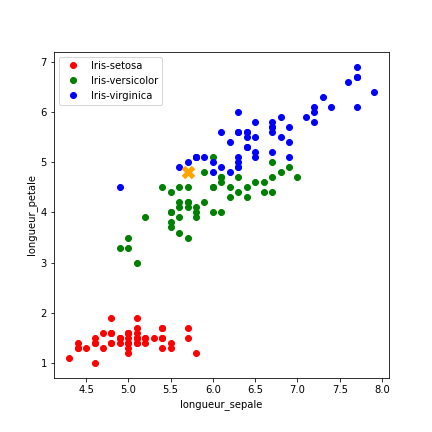
\includegraphics[width=1\textwidth,height=\textheight]{images/iris-longpetale-longsepale-point.png}\\
\emph{Graphique 1 : Jeu de données iris avec deux descripteurs}

\end{minipage} \end{tabular}

\end{center}

\begin{enumerate}
\def\labelenumi{\arabic{enumi}.}
\setcounter{enumi}{3}
\item
  Avec la fonction \passthrough{\lstinline!afficher\_donnees\_point!} du
  module \passthrough{\lstinline!utilitaires\_knn!}, afficher le jeu de
  données et la nouvelle donnée dans un repère du plan en repérant les
  points par trois descripteurs
  \passthrough{\lstinline!"longueur\_sepale"!},
  \passthrough{\lstinline!"longueur\_petale"!} et
  \passthrough{\lstinline!"largeur\_sepale"!}. On doit obtenir le
  graphique 2.

  \begin{itemize}
  \tightlist
  \item
    Les trois nuages de points classés par espèce sont-ils bien séparés
    ? L'algorithme des k plus proches voisins va-t-il bien fonctionner
    en général ?
  \item
    Le point marqué d'une croix orange représente l'iris d'espèce
    inconnue. L'algorithme des k plus proches voisins va-t-il bien
    fonctionner pour cet iris particulier ?
  \item
    Avec la fonction \passthrough{\lstinline!etiquetage\_knn!}, écrire
    un code qui affiche les prédictions de l'algorithme des k plus
    proches voisins pour k variant entre 1 et 20. Comparer avec les
    résultats obtenus à la question 3. avec deux descripteurs.
  \end{itemize}
\end{enumerate}

\begin{center}

\begin{tabular}{c}

\begin{minipage}{0.8\linewidth}

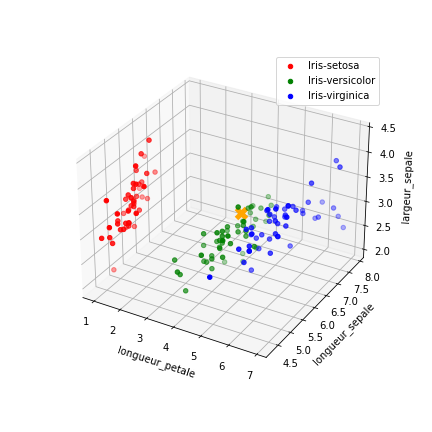
\includegraphics[width=1\textwidth,height=\textheight]{images/iris-larsetale-longsepale-longpetale-point.png}\\
\emph{Graphique 2 : Jeu de données iris avec trois descripteurs}

\end{minipage} \end{tabular}

\end{center}

\hypertarget{distance-de-manhattan-optimisation-de-la-complexituxe9-puis-uxe9tude-de-linfluence-du-paramuxe8tre-k}{%
\section{Distance de Manhattan, optimisation de la complexité puis étude
de l'influence du paramètre
k}\label{distance-de-manhattan-optimisation-de-la-complexituxe9-puis-uxe9tude-de-linfluence-du-paramuxe8tre-k}}

Dans la ville imaginaire de Manhattan, les rues sont agencées selon un
quadrillage et la distance entre deux immeubles A et B de coordonnées
\((x_{A},y_{A})\) et \((x_{B},y_{B})\) correspond à la longueur du
parcours d'un taxi allant de A vers B en longeant les rues :
\(distanceManhattan(A, B)=\vert x_{B} - x_{A} \vert + \vert y_{B} - y_{A} \vert\).

On considère que chaque immeuble de la ville sont repérés dans un repère
orthonormé par un couple de coordonnées \((x, y)\) où \(x\) et \(y\)
sont des entiers naturels.

Dans répertoire \passthrough{\lstinline!datas!} qui est fourni, se
trouve un fichier \passthrough{\lstinline!nettoyage.csv!} avec 944
enregistrements d'immeubles de Manhattan avec trois descripteurs `x',
`y' et une étiquette `nettoyage' :

\begin{itemize}
\tightlist
\item
  `x' : abscisse de l'immeuble un entier compris entre 0 et 100
\item
  `y' : ordonnée de l'immeuble un entier compris entre 0 et 100
\item
  `nettoyage' : le nom de l'entreprise de nettoyage de l'immeuble qui
  peut prendre deux valeurs : `jules' ou `paul'
\end{itemize}

On travaille toujours dans le fichier
\passthrough{\lstinline!tp\_eleve.py!}.

\begin{enumerate}
\def\labelenumi{\arabic{enumi}.}
\tightlist
\item
  Saisir le code suivant pour :
\end{enumerate}

\begin{itemize}
\tightlist
\item
  charger dans une variable \passthrough{\lstinline!table\_nettoyage!}
  le contenu du jeu de données \passthrough{\lstinline!nettoyage.csv!}
  avec la fonction \passthrough{\lstinline!charger\_fichier\_entete!} du
  module \passthrough{\lstinline!utilitaires\_knn!} ;
\item
  afficher le jeu de données et enregistrer l'image dans le répertoire
  de travail.
\end{itemize}

\begin{lstlisting}[language=Python]
table_nettoyage = charger_fichier_entete('./datas/nettoyage.csv')
afficher_donnees(["x", "y"], 
                 'nettoyage', table_nettoyage, 
                 fichier = 'nettoyage.png')
\end{lstlisting}

\begin{center}

\begin{tabular}{c}

\begin{minipage}{0.8\linewidth}

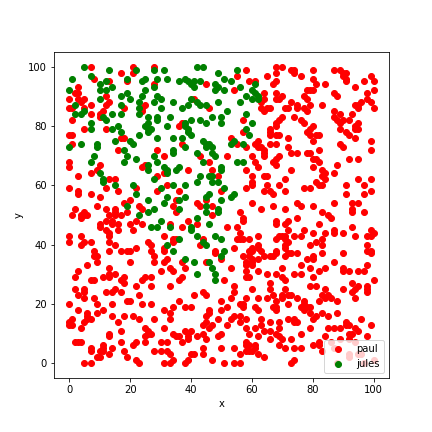
\includegraphics[width=0.8\textwidth,height=\textheight]{images/nettoyage.png}\\
\emph{Graphique 3 : Entreprises de nettoyages dans Manhattan}

\end{minipage} \end{tabular}

\end{center}

\begin{enumerate}
\def\labelenumi{\arabic{enumi}.}
\setcounter{enumi}{1}
\tightlist
\item
  Compléter le code de la fonction
  \passthrough{\lstinline!distance\_manhattan!} en respectant la
  spécification donnée dans la \passthrough{\lstinline!docstring!}.
  Vérifier ensuite que le test unitaire
  \passthrough{\lstinline!test\_unitaire\_distance\_manhattan()!} est
  réussi.
\end{enumerate}

\begin{lstlisting}[language=Python]
def distance_manhattan(enreg_a, enreg_b, tab_descripteur):
    """
    Parameters
    ----------
        enreg_a, enreg_b et deux enregistrements de données sous forme de 
        dictionnaires
        tab_descripteur un tableau de descripteurs (certaines clefs des 
                                                    enregistrements)
    
    Returns
    -------
        distance de manhattan entre enreg_a et enreg_b selon les valeurs des 
        descripteurs de tab_descripteur arrondie à 3 chiffres après la virgule
    """
    distance = 0
    for descripteur in tab_descripteur:
        distance = "à  compléter"
    return distance
\end{lstlisting}

\begin{enumerate}
\def\labelenumi{\arabic{enumi}.}
\setcounter{enumi}{2}
\tightlist
\item
  Compléter le code suivant afin d'afficher une prédiction de
  l'entreprise de nettoyage choisie pour un nouvel immeuble de
  coordonnées \((30, 43)\), à l'aide de la fonction
  \passthrough{\lstinline!etiquetage\_knn!} écrite précédemment. On
  pensera à passer en paramètre la fonction
  \passthrough{\lstinline!distance\_manhattan!} car la distance par
  défaut est \passthrough{\lstinline!distance\_euclidienne!}. Pour
  simplifier on suppose que si un immeuble existe déjà au point de
  coordonnées \((30, 43)\) alors une nouvelle étiquette est attribuée.
\end{enumerate}

\begin{lstlisting}[language=Python]
nouveau_client = {'x' : 30, 'y' : 43}
for k in range(1, 11):
    prediction = "à compléter"
    print("k = ", k, "prédiction  :", prediction)
\end{lstlisting}

\begin{enumerate}
\def\labelenumi{\arabic{enumi}.}
\setcounter{enumi}{3}
\tightlist
\item
  La complexité temporelle dominante dans l'algorithme des k plus
  proches voisins que nous avons implémenté est celle du tri, ce qui
  donne un ordre de grandeur en \(n \log(n)\) pour un jeu de données de
  taille \(n\). On va implémenter un algorithme de complexité linéaire,
  d'ordre de grandeur \(n\), ce qui sera plus performant sur des jeux de
  données de très grande taille
\end{enumerate}

\begin{itemize}
\tightlist
\item
  On considère un algorithme de complexité en \(n \log(n)\) (fonction
  logarithme décimal de la calculatrice qui donne approximativement le
  nombre de chiffres d'un nombre en base dix) et on admet que son temps
  d'exécution pour un jeu de données de taille \(n=10\) est de 1
  milliseconde. Quel est son temps d'exécution pour un jeu de données de
  taille \(1000\) ? de taille \(100000\) ? de taille \(10^{6}\) ?
\item
  On considère un algorithme de complexité en \(n \log(n)\) et on admet
  que son temps d'exécution pour un jeu de données de taille \(n=10\)
  est de 2 millisecondes. Quel est son temps d'exécution pour un jeu de
  données de taille \(1000\) ? de taille \(100000\) ? de taille
  \(10^{6}\) ?
\item
  Quel est l'intérêt d'une complexité en \(n\) par rapport à une
  complexité en \(n \log(n)\) ?
\end{itemize}

\begin{enumerate}
\def\labelenumi{\arabic{enumi}.}
\setcounter{enumi}{4}
\tightlist
\item
  Pour obtenir un algorithme de complexité linéaire,on ne va pas trier
  tout le jeu de données de taille \(n\) mais maintenir une liste les k
  plus proches voisins lors du parcours du tableau
  \passthrough{\lstinline!tab\_distance!}.
\end{enumerate}

Celui-ci contient les tuples (distance, étiquette) sous cette forme :

\begin{lstlisting}[language=Python]
[(10.0, 'paul'), (13.0, 'paul'), (14.0, 'paul'), (16.0, 'jules'), (17.0, 'paul'), ...]
\end{lstlisting}

On procède ainsi :

\begin{itemize}
\tightlist
\item
  On trie d'abord les k premiers éléments de
  \passthrough{\lstinline!tab\_distance!} dans une liste
  \passthrough{\lstinline!k\_voisins!}
\item
  Pour chacun des couples suivants on l'insère à sa place dans
  \passthrough{\lstinline!k\_voisins!} puis on enlève le dernier élément
  de \passthrough{\lstinline!k\_voisins!} (de plus grande de distance)
  pour garder uniquement les k voisins les plus proches. L'algorithme
  d'insertion est le même que pour le tri par insertion.
\end{itemize}

Compléter la fonction
\passthrough{\lstinline!trier\_puis\_extraire\_insertion!}.

Vérifier avec le test unitaire
\passthrough{\lstinline!test\_unitaire\_trier\_puis\_extraire\_insertion()!}.

\begin{lstlisting}[language=Python]
def trier_puis_extraire_insertion(tab_distance, k):
    """
    Parameters
    ----------
    tab_distance un tableau de tuple (distance entre deux  enregistrements
    , étiquette) renvoyé par table_distance_nouveau
    
    Returns
    -------
    tableau k_voisins des k plus petits éléments de tab_distance
    selon le critère de distance
    """
    #précondition
    assert k <= len(tab_distance)
    #liste triée des k premiers tuples de tab_distance 
    k_voisins = sorted([tab_distance[i] for i in range(k)])
    #parcours des tuples suivants
    for i in range(k, len(tab_distance)):     
        nouveau = tab_distance[i]
        #ajout de nouveau à la fin de tab_distance
        k_voisins.append(nouveau)
        #insertion de nouveau à sa place dans la liste triée k_voisins
        #comme dans le tri par insertion avec une boucle while
        j = k - 1
        "à compléter"
        
        
        
        #invariant : ici k_voisins toujours dans l'ordre croissant des distances
        #on enlève le  dernier tuple de k_voisin = voisin le plus loin
        k_voisins.pop()
    #on extrait de k_voisins la liste des étiquettes uniquement
    return [voisin[1] for voisin in k_voisins[:k]]
\end{lstlisting}

Modifier la fonction \passthrough{\lstinline!etiquetage\_knn!} en une
fonction \passthrough{\lstinline!etiquetage\_knn\_insertion!} qui prédit
une étiquette en utilisant
\passthrough{\lstinline!trier\_puis\_extraire\_insertion!}.

\begin{enumerate}
\def\labelenumi{\arabic{enumi}.}
\setcounter{enumi}{5}
\tightlist
\item
  On veut mesurer expérimentalement la complexité temporelle de
  \passthrough{\lstinline!etiquetage\_knn\_insertion!}. Spécifier la
  fonction \passthrough{\lstinline!mesure\_temps!} qui est fournie. à
  l'aide d'une \passthrough{\lstinline!docstring!}.
\end{enumerate}

On donne ci-dessous un exemple d'exécution. Commenter les résultats
affichés.

\begin{lstlisting}[language=Python]
In [43]: mesure_temps(etiquetage_knn_insertion, 5)
Taille :  100  Temps :  0.0001652430000831373 Ratio = temps/ temps_precedent = None
Taille :  1000  Temps :  0.0013811469998472603 Ratio = temps/ temps_precedent = 8.358278409084654
Taille :  10000  Temps :  0.01579672799925902 Ratio = temps/ temps_precedent = 11.437398047424324
Taille :  100000  Temps :  0.15101633700032835 Ratio = temps/ temps_precedent = 9.559975775199275
Taille :  1000000  Temps :  1.513596802999018 Ratio = temps/ temps_precedent = 10.022735507057936
\end{lstlisting}

\begin{enumerate}
\def\labelenumi{\arabic{enumi}.}
\setcounter{enumi}{6}
\tightlist
\item
  On fournit une procédure d'en-tête
  \passthrough{\lstinline!influence\_k(nb\_clients,  cote\_ville)!} qui
  prédit l'étiquette pour tous les immeubles de la ville avec
  l'algorithme des k plus proches voisins, k variant de 1 à 10 et
  affiche la carte des prédictions. Si l'immeuble est déjà dans le jeu
  de données on fait quand même une prédiction , qui peut être
  différente de l'étiquette du point (pas absurde si on le voit comme
  une réattribution de marché). Exécuter le test proposé puis commenter
  à partir des images obtenues l'influence du paramètre k sur la
  prédiction. Un exemple en video est disponible
  \href{\%5Bimages/KNN-Influence-de-k.gif\%5D(https://nuage03.apps.education.fr/index.php/s/Re7CtAHmEN4yTy3)}{ici}
\end{enumerate}

\begin{center}

\begin{tabular}{cc}

\begin{minipage}{0.5\linewidth}

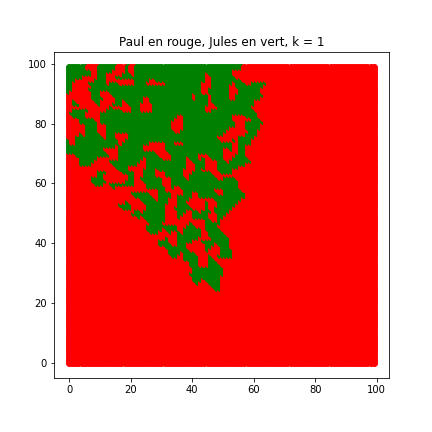
\includegraphics[width=1\textwidth,height=\textheight]{images/influence-k=1.png}\\

\end{minipage} &

\begin{minipage}{0.5\linewidth}

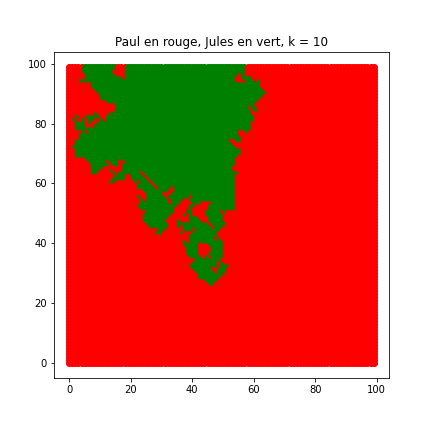
\includegraphics[width=1\textwidth,height=\textheight]{images/influence-k=10.png}\\

\end{minipage} \end{tabular}

\end{center}

\emph{Graphique 4 : Influence du paramètre k}

\end{document}
